\section{Et la température dans tout ça ? (4 points)}

Le graphique ci-dessous représente la solubilité du  sel (ou chlorure de sodium) dans l'eau en fonction de la température.

\begin{questions}
	\question[2] Complète le graphique en indiquant les grandeurs représentées ainsi que leurs unités en abscisse et en ordonnée.
	
	\begin{center}
		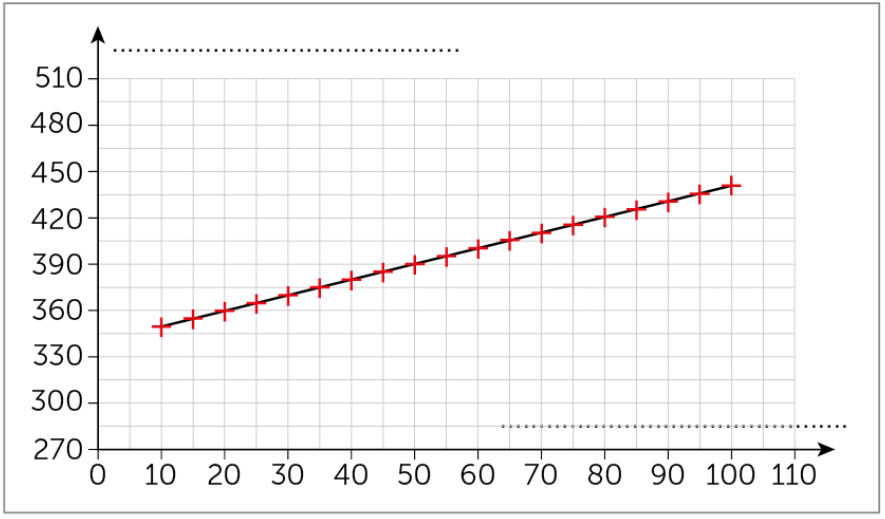
\includegraphics[scale=0.7]{img/courbe}
	\end{center}

	\question[1] \`A $20 $°$C$, quelle masse de chlorure de sodium peut-on dissoudre au maximum dans 1L de solution ?
	
	\question[1] \`A $90 $°$C$, quelle masse de chlorure de sodium peut-on dissoudre au maximum dans 1L de solution ?
	
	\question[1] De quoi dépend la solubilité du sel dans l'eau ?
\end{questions}
